\documentclass{article}

\usepackage[margin=1.5in]{geometry}
\usepackage{authblk}          % For 2+ authors
\usepackage{mathtools}        % an improvement that incorporates amsmath.
\usepackage{comment}
\usepackage[ruled,noline]{algorithm2e}
\usepackage{url}              % Used for linkable URLs.
\usepackage{pgfplots}
\usepackage{changepage}       % Used to adjust the margins for wide tables.

\pgfplotsset{compat=1.16}
% Empty Square Brackets are used to mean empty intervals.
\newcommand{\esb}{[\,]}

\begin{document}
\title{Partition Maps}
\author{Leonid Rozenberg\thanks{leonidr@gmail.com}}
\date{}                             % Supress printing the date under the title.
\maketitle

\begin{abstract}
  A partition map is a data structure to represent functions where we
  privilege merging,
  generating new functions,
  above other operations.
  I motivate the use of partition maps in lieu of other data structures
  and describe challenges in implementing the necessary logic.
\end{abstract}

\section{Introduction}

A mathematician can think of a partition map as a way to represent a function
($f : D \rightarrow R$), an association, a map.
A programmer can think of it as a way to track, non-scalar
state\footnote{I will mix the two nomenclatures and ways of thinking
as domain and range are particularly succinct and useful terms.}.

There are many data structures that one can use to represent functions,
or state,
such as arrays, association lists, trees, hash tables and variants of these.
The deciding factor of which implementation to use depends upon the stored
data and desired access pattern.
Most data structures privilege value setting and getting;
accessing and mutating the value associated with any key in the domain.
A partition map, is a different technique,
where we prioritize \emph{merging} above other access patterns.

As a running motivating example,
let $D$ be the positive integers up to $100$,
and consider the functions

\begin{minipage}{.5\linewidth}
\begin{displaymath}
  f_{1}(x) = \left\{
        \begin{array}{c c}
          1 & x \in [10,80] \\
          0 & \text{otherwise,} \\ %x \in [1,9] \cup [91,100] \\
        \end{array}
     \right.
\end{displaymath}
\end{minipage}%
\begin{minipage}{.5\linewidth}
\begin{displaymath}
  f_{2}(x) = \left\{
        \begin{array}{c c}
          1 & x \in [20,90] \\
          0 & \text{otherwise.} \\ %x \in [1,9] \cup [91,100] \\
        \end{array}
     \right.
\end{displaymath}
\end{minipage}
Merging takes two functions and computes a new
one
such as
\begin{displaymath}
  g(x) = f_{1}(x)+f_{2}(x) = \left\{
        \begin{array}{c c}
          0 & x \in [1,9] \cup [91,100] \\
          1 & x \in [10,19] \cup [81,90] \\
          2 & x \in [20,80]. \\
        \end{array}
     \right.
\end{displaymath}

The range, $R$, is specified by each function.
It may vary, but for our purposes I want to emphasize that it is smaller
than the domain.
Lastly,
we are not concerned with composition,
cases such as $g(x)=f_{j}(f_{i}(x))$.

Briefly, as a point of comparison,
consider the storage and merging costs for various data
structures that could be used to model $f_{1}, f_{2}$ and then create $g$.
An array, where we use one array position for each element in the domain,
would require $O(|D|)$ storage and $O(|D|)$ evaluations for merging.
This is the naive case.
We can have similar performance using other data-structures
(lists, trees and hash-tables) following the naive approach,
one value per domain element,
but with the extra overhead of pointer management.

A couple of the conditions,
present in the example,
should highlight what is inefficient about the naive solution.
%These conditions are the ones that partition maps aims to address.
\begin{enumerate}
  \item The size of the range ($R$) is much smaller than the domain ($D$).
    For $f_{1}$ or $f_{2}$ we have 2 elements vs $100$,
    and for $g$ the case is $3$ vs $100$.
    The specific relation of the two values is not as important as emphasizing
    that we want to create bounds proportional to $|R|$ as opposed to $|D|$.

  \item Traditionally,
    when programmers are concerned with excessive or redundant evaluations,
    they will use memoization.
    In this case it is dubious that it will improve the situation as
    performing the calculation
    is so simple that it might be cheaper than looking up the result.
    Thus, the merging operation is \emph{simple}\footnote{
      These terms are unfortunately left imprecise at the moment as making
      them precise is part of the ongoing effort.}.

  \item The merging operation is \emph{bounded}\footnote{Ibid.},
    it does not grow the size of the range excessively.
    An example of a function that grows excessively would be $h(x) = x + f_{1}$.
    If we know that all \emph{future} merging operations are also bounded,
    we are even more motivated to merge in $O(|R|)$ time.

  \item The domain is fixed.
    We know the full state for which we want to keep track of values and it
    does not change.
    Many algorithms that we might use instead assume,
    \emph{a priori} that the user does not know the full domain,
    consequently concerning themselves with how it might grow or shrink.

\end{enumerate}

Usually,
we think about such problems by allocating space sufficient for our domain
and then operate on each element therein.
But if we know that the range is much smaller,
it will not grow much in size,
and the domain is known ahead of time,
can we do better?
Specifically,
can we operate over the range elements,
and add extra bookkeeping operations to track the domain elements,
that will make the resulting code faster?

For each function that we specify,
working backwards,
the values in the range specify a partition of the domain.
For example,
for $g$, $S_{0} = [1,9]\cup [91,100], S_{1} = [10,19] \cup [81,90], S_{2} = [20,80]$
and $S_{0} \cup S_{1} \cup S_{2} = D = [1,100]$.
I will refer to this as the partition \emph{implied} by a function.

For the functional language enthusiast, the \emph{merge} that I
describe is commonly thought of as a \emph{map2}; a higher order function that
takes another function $m$ that is applied to each element of two other
structures,
where the arguments to $m$,
are chosen based on the internals of the data structures.
I eschew that name to emphasize that something different,
something dependent on the domain elements,
will occur when we merge.
Moreover, \emph{map} will have a slightly different interpretation.
When we \emph{map},
we consider all of the unique elements of the range and
apply a function to each of these values,
with two caveats: the transform does not take a domain element as an
argument and we store only the unique elements of the resulting range.
Similarly, when we merge we will again ignore the domain elements when computing
the new value,
keep track of only the unique resulting values,
but also take elements from the two ranges such that their respective domain sets
have an intersection.

\section{Example applications}

It is important to stress that these conditions are unique to the problem that
I encountered and may not be present in other scenarios.
To give more motivation for this method it might be worthwhile to consider
potential applications.

\subsection{Histograms}

The functions that I used as my motivating examples might seem like toy
examples without actual use.
In practice,
functions that are only a little bit more complicated,
can arise when a user wants to track an empirical distribution with a histogram.
Or even simpler uses such as frequency tables.
One of the most common first steps in the construction of such tables is to
decide the number of classes or bins;
how to partition the domain.
What if that was a question that was largely determined empirically?

This approach could have positive benefits in systems that want to integrate
statistics from different observations, via such histograms.
Distributed systems come to mind.
For example, different routers might keep a map of packet size to latency
(or other metric).
But the domain space,
packet size,
could have a clustering effect
where packets that have nearly the same size
(eg. 100 or 105 bytes),
have the same outcome.
Or a large threshold effect,
if a packet is larger than 1kb then it's metric is twice the value of
those below.
In both cases,
a partition map would provide a sparser representation,
and potentially simpler merging logic for aggregating algorithms.

\subsection{Columnar Store}

As another example consider merging columns of discrete values,
in a table,
such as a credit calculation.
There are several columns all indexed by the same primary key UserId.
\begin{center}
\begin{tabular}{|r|l|l|l|l|}
\hline
  UserId & Education   & Income Bracket & Age Group & Credit \\
\hline
  1      & High School & $<10k$       & $< 20$  & Bad    \\
  2      & High School & $<10k$       & $< 20$  & Bad    \\
  \ldots & \ldots      & \dots        & \ldots  & \ldots \\
  103    & High School & $<10k$       & 20-30   & Bad    \\
  104    & High School & $<10k$       & 20-30   & Bad    \\
  \ldots & \ldots      & \dots        & \ldots  & \ldots \\
  206    & High School & $10k-50k$    & 20-30   & Bad    \\
  %\ldots & \ldots      & \dots        & \ldots  & \ldots \\
  %706    & Bachelors   & $<10k$       & 20-30   & Bad    \\
  \ldots & \ldots      & \dots        & \ldots  & \ldots \\
  1506   & Bachelors   & $50k-100k$   & 20-30   & Ok     \\
  \ldots & \ldots      & \dots        & \ldots  & \ldots \\
  %6506   & Bachelors   & $>100k$      & 30-40   & Ok \\
  %\ldots & \ldots      & \dots        & \ldots  & \ldots \\
  11986  & Bachelors   & $>200k$      & 30-40   & Good \\
  \ldots & \ldots      & \dots        & \ldots  & \ldots \\
  252321 & Doctorate   & $50k-100k$   & 20-30   & Ok \\
  \ldots & \ldots      & \dots        & \ldots  & \ldots \\
  \hline
\end{tabular}
\end{center}
In this example, all of the inputs to our merge function
(eg. Education can be one of ``High School'', ``Bachelors''
or ``Doctorate'').
and the output (Credit can be either Good, Medium or Bad)
are discrete.
If the individual datums are stored independently (eg. we have not
already allocated the full table to store the data and result) a
partition map approach might be warranted.

\subsection{Original motivation}

My objective,
when developing partition maps,
was to compute a likelihood function,
a probability for a large set of genetic variants.
The likelihood function was computed via a sequence of multiple recursions,
in a dynamic programming approach.

\begin{align}
  M_{lkn} &= e_{lkn}(t_{MM}M_{l-1,k,n} + t_{IM}I_{l-1,k,n} + t_{DM}D_{l-1,k,n})
  \nonumber \\
  I_{lkn} &= \frac{1}{4}(t_{MI}M_{l-1,k,n} + t_{II}I_{l-1,k,n}) \nonumber \\
  D_{lkn} &= t_{MD}M_{l,k,n} + t_{DD}D_{l,k,n} \nonumber
\end{align}

The genetic variants (the state/domain space indexed by $n$),
were similar in many instances and the functions were
bounded by their numerical accuracy.
The calculations were also simple,
a cross product of probabilities ($M, I, D$) and weights ($t_{MM}, t_{IM}, t_{DM} \ldots$).
The application had to perform this calculation several million times
per sample.
This was a big computational bottleneck
and performing this computation via partition maps
reduced the running time to less than 5\% of the naive approach.


\section{Related approaches}

Before describing the implementation it would be helpful to quickly survey the
literature of related data structures;
to contrast how they do not meet the requirements and
for inspiration.
The common refrain is that they will make an undesired trade-off,
where they favor look-ups versus merging.

\subsection{Bidirectional maps}

A bidirectional map\footnote{\url{https://en.wikipedia.org/wiki/Bidirectional_map}},
can be thought of as set whose elements are pairs that represent the association,
coupled with lookup and alteration methods so that the set (maps) is (are) preserved
regardless of which side is used as a key.
For our purposes, naively, they would require storing an element of the domain.
Non-naively, if one side was to represent a set of the implied partition,
we are still willing to discard the convenience of look-ups for fast merges.

\subsection{Fast Mergeable Integer Maps}

Okasaki's classic description\cite{Okasaki1998} of Patricia trees highlights how
we can maximize the information contained within keys to build efficient data
structures.
Unfortunately, for our purposes, this technique has a slightly different
interpretation of \emph{merging},
combining disparate sets of keys and values that preserve fast lookup.
We intent to merge two cases where values for all the keys are already known.

One could imagine mapping every set within a partition to a unique, large,
integer by representing it as a bit vector (a bit per element), and then
utilizing Patricia tree's as described in this work.
The large key sizes ($O(|D|)$ bits),
pose a substantial problem as the bit-twiddling necessary for look-ups is
limited to a programs word size which might be a relatively small portion
of $|D|$.
Furthermore, the original fast lookup guarantees provided by the integers are
now swamped by this bigger size.
Lastly, this method, like the others described, does not utilize our previous
knowledge of a fixed domain.

One potential way to rescue this work would be an effective,
possibly probabilistic,
hash of sets in a partition to integers.

\subsection{DIET}

Discrete Interval Encoding Trees\cite{Erwig1993},
describe an efficient representation for sets of types that are easily
transformed into integers.
The use of intervals to represent sets is an affirmation of my approach.
Sadly, it is far from straightforward to figure out how to adapt these
sets to represent maps,
they will break the adjacency of nearby intervals.
Finally,
while traversing the leaf nodes of a tree is not difficult,
constructing trees in that order can lead to pathological cases.
At the end of the day,
I am not certain that trees provide the right storage organization for our use
case.

\subsection{Mergeable Interval Map}

The Mergeable Interval Map\cite{Bonichon2010} cleverly extends Okasaki's
technique to ranges of integers, in the style of DIETs.
This work is probably closest in spirit to the
data structure that I intent to describe but the focus on retrieval,
even if optimized for arbitrary intervals,
is not the trade-off that I seek.

\section{A non-naive implementation}

A non-naive solution seeks smaller costs than one value per domain element.
Arrays are not amenable to such approaches
because the association between domain and range is implicit;
each position in the array is associated with an element from the domain
based on some enumeration.
What is stored in each position is then the appropriate element in the range.

An association list is a linked list where each node contains a key and a value.
They allow us $O(|R|)$ storage since we can store just one value per node.
The problem then turns into how to represent and order the keys,
the sets of a partition of $D$ implied by $f$.
For the moment,
let us assume that we have such a representation,
$S_{i}$, and order.
For $f_{1}$, $S_{1} = [10,80]$ and $S_{2} = [1,9]\cup[81,100]$.
There is a simple algorithm (Alg.\ref{Alm1}) to merge two association lists.
Traverse both lists looking for intersections between the sets.
If an intersection between the keys exists,
merge the two values and then insert that,
keyed by the intersection,
into an association list accumulator.

\begin{algorithm}[H]
  \SetKwProg{Fn}{Function}{\string:}{}
  \newcommand{\forcond}{$i=0$ \KwTo $n$}
  \SetKwFunction{Merge}{Merge1}%
  \SetKwFunction{Insert}{InsertIntoList}%
  \DontPrintSemicolon
  \Fn(){\Merge{$L_{1}, L_{2}, f$}}{
    \KwData{Two association lists, $L_{1}, L_{2}$, and the merge function, $f$.}
    \KwResult{$L$ merged association list.}
    % Unlike square brackets this looks fine without an extra space.
    $L \leftarrow \{\} $\;
    \ForEach{$S_{1},v_{1} \in L_{1}$}{
      $R \leftarrow S_{1}$\tcp*[r]{Remaining}
      \ForEach{$S_{2},v_{2} \in L2$ \textup{and} $R \neq \emptyset$}{
        \lnlset{inter}{inter}$I \leftarrow R \cap S_{2}$\;
        \lnlset{diff}{diff}$R \leftarrow R \backslash S_{2}$\;
        \uIf{$I \neq \emptyset$}{
          \Insert{$I,v,L$}\;
        }
      }
    }
    Sort $L$ by keys, the sets
    \Return{$L$}
  }
  \Fn(){\Insert{$I, v, L$}}{
    \KwData{A set $I$, the key of value $v$ and $L$, a list to insert into.}
    \KwResult{Modifies $L$, the lead pointer does not change.}
    \ForEach{$S_{i},v_{i} \in L$}{
      \uIf{$v_{i} = v$}{
        $S_{i} \leftarrow S_{i} \cup I$\tcp*[r]{Modify the set}
        \Return
      }
    }
    Append $(I,v)$ to end of $L$.\;
  }
\caption{Merging Two Association Lists.\label{Alm1}}
\end{algorithm}

The rub is in how we insert the new keyed value into the accumulator.
One sensible strategy would be to prepend (cons) each set-value pair to the
front of the accumulator after we find an intersection.
While this is the fastest approach it does not bind the growth of the
association list.
In order to enforce that the association list contains only unique values
we have to traverse the entire accumulator.
If $L_{1}$ and $L_{2}$ have $m, n$ elements respectively,
and consider the worst case that the function creates no duplicate values,
this leads to a pretty disappointing $O(n^{2}m^{2})$ running time.
This running time also excludes the set intersection and difference
operations (labeled lines \ref{inter} and \ref{diff} in the algorithm),
as if they were not expensive.

But they are expensive.
One initially suitable approach to representing the $S_{i}$ would be
to use a bit vector.
This is a common, well understood, data-structure,
especially as the algorithms to compute set intersection and difference require
simple bitwise logic operators.
The problem is that this bit vector would still require $|D|$ bits,
and $O(|D|)$ operations.

The solution that I propose is to use pairs to represent the sequential,
inclusive intervals that cover each $S_{i}$ stored in \emph{ascending} order.
The intervals partition the set $[1,|D|]$,
representing the domain,
using the same representation as the one if storing $D$ in an array.

For example\footnote{I am using square brackets ([]) to denote
intervals (and pairs) and curly brackets (\{\}) to denote lists.
This is counter to many common functional programming languages,
but it reinforces the mathematical notation.
Using parentheses for intervals would be confusing as I explicitly want to
use inclusive intervals.},
for $f_{1}$, $S_{0} = \{[1,9],[81,100]\}$ and $S_{1} = \{[10,80]\}$
and for $g$, $S_{0} = \{[1,9], [91,100]\}$,
$S_{1} = \{ [10,19], [81,90]\}$,
and $S_{2} = \{[20,80] \}$
This approaches main advantage is that it allows us to escape from $O(|D|)$
as each $S_{i}$ is bounded by $|R|$.

Using intervals has other advantages over bit vectors.
Computing the intersection and difference requires a straight-forward
but large case analysis of the ways that two intervals can
intersect (Algorithm \ref{Alm2}),
that needs simple integer comparison.
Because our key elements are discrete we know our borders exactly.

\begin{algorithm}[H]
  \DontPrintSemicolon
  \SetKwProg{Fn}{Function}{\string:}{}
  \newcommand{\forcond}{$i=0$ \KwTo $n$}
  \SetKwFunction{Iiad}{IntervalIntersectionDifference}
  \Fn(){\Iiad{$I_{1}, I_{2}$}}{
    \KwData{Two intervals $I_{1} = [s_{1},e_{1}]$ and $I_{2}=[s_{2},e_{2}]$
      of non-negative integers that are non-empty,
      $s_{1} \leq e_{1}$ and
      $s_{2} \leq e_{2}$.}
    \KwResult{A quintuple of potentially empty ($\esb$)
      intervals: the intersection,
      the part of $I_{1}$ that come before the intersection\footnote{Even though
      the intersection may be empty (such as the first case) $I_{1}$ or $I_{2}$
      may still be before it in the sense that they are before the midpoint.
      The same interpretation applies to the parts that come after an
      intersection (such as the last case).},
      the part of $I_{2}$ that come before the intersection,
      the part of $I_{1}$ that come after the intersection,
      and the part of $I_{2}$ that come after the intersection.
      }
      \uIf{$s_{2} < s_{1}$}{
        \uIf{$e_{2} < s_{1}$}{
          \Return $\esb,\esb,I_{2},I_{1},\esb$
        }\uElseIf{$e_{2} < e_{1}$}{
          \Return $[s_{1}, e_{2}],\esb,[s_{2},s_{1} - 1], [e_{2} + 1, e_{1}], \esb$
        }\uElseIf{$e_{2} = e_{1}$}{
          \Return $I_{1},\esb, [s_{2}, s_{1} - 1], \esb,\esb$
        }\uElse(\tcp*[h]{$e_{2} > e_{1}$}){
          \Return $I_{1}, \esb, [s_{2}, s_{1} - 1],\esb, [e_{1} + 1, e_{2}]$
        }
      }
      \uElseIf(\,\tcp*[h]{$e_{2} \geq s_{1}$}){$s_{2} = s_{1}$}{
        \uIf{$e_{2} < e_{1}$}{
          \Return $[s_{1}, e_{2}], \esb,\esb, [e_{2} + 1, e_{1}],\esb$
        }\uElseIf{$e_{2} = e_{1}$}{
          \Return $ I_{1},\esb,\esb,\esb,\esb$
        }\uElse(\tcp*[h]{$e_{2} > e_{1}$}){
          \Return $I_{1},\esb,\esb,\esb,[e_{1} + 1, e_{2}]$
        }
      }
      \uElseIf(\,\tcp*[h]{$e_{2} > s_{1}$}){$s_{1} < s_{2}$ \textup{and} $s_{2} < e_{1}$}{
        \uIf{$e_{2} < e_{1}$}{
          \Return $I_{2},[s_{1}, s_{2}-1],\esb,[e_{2}+1, e_{1}],\esb$
        }\uElseIf{$e_{2} = e_{1}$}{
          \Return $I_{2}, [s_{1}, s_{2}-1],\esb,\esb,\esb$
        }\uElse($ e_{2} > e_{1} $){
          \Return $[s_{2}, e_{1}], [s_{1}, s_{2}-1],\esb,\esb, [e_{1} + 1, e_{2}]$
        }
      }
      \uElseIf(\,\tcp*[h]{$ e_{2} \geq e_{1}$}){$e_{1} = s_{2}$}{
        \uIf{$e_{2} = e_{1}$}{
          \Return $I_{2}, [s_{1}, s_{2} - 1], \esb,\esb,\esb$
        } \uElse(\tcp*[h]{$e_{2} > e_{1}$}){
          \Return $[s_{2}, e_{1}], [s_{1}, s_{2} - 1], \esb,\esb,[e_{1} + 1, e_{2}]$
        }
      }
      \uElse(\tcp*[h]{$e_{1} < s_{2}$}){
        \Return $\esb,I_{1},\esb,\esb,I_{2}$
      }

  }
\caption{Interval Intersection and Difference.\label{Alm2}}
\end{algorithm}

% Reconsider this page break if we can have a nicer position for the algorithm
\pagebreak

The interval intersection-difference operation is then coupled with a fold
over the two lists that contain the entire set.

\begin{algorithm}[H]
  \SetKwProg{Fn}{Function}{\string:}{}
  \newcommand{\forcond}{$i=0$ \KwTo $n$}
  \SetKwFunction{Iad}{IntersectionAndDifference}%
  \SetKwFunction{Iiad}{IntervalIntersectionDifference}%
  \DontPrintSemicolon
  \Fn(){\Iad{$S_{1}, S_{2}$}}{
    \KwData{Two lists of \emph{ascending} intervals $S_{1}, S_{2}$.}
    \KwResult{A list of intersecting interval $S_{i}$, and two lists of the
      set differences for each input lists $S_{d1}
      %(\forall x \in S_{1} \wedge \notin S_{2})
      , S_{d2}$.}
    $S_{i} \leftarrow \{ \} $\;
    $S_{d1} \leftarrow \{ \} $\;
    $S_{d2} \leftarrow \{ \} $\;
    \While{$S_{1} \neq \{ \}$ \textup{and} $S_{2} \neq \{ \} $}{
      $I_{1} \leftarrow $ pop first element of $S_{1}$\;
      $I_{2} \leftarrow $ pop first element of $S_{2}$\;
      $I, B_{1}, B_{2}, A_{1}, A_{2} \leftarrow$ \Iiad{$I_{1}, I_{2}$}\;
      \lIf{$I \neq \esb$}{ Append $I$ to end of $S_{i}$}
      \lIf{$B_{1} \neq \esb$}{ Append $B_{1}$ to end of $S_{d1}$}
      \lIf{$B_{2} \neq \esb$}{ Append $B_{2}$ to end of $S_{d2}$}
      \lIf{$A_{1} \neq \esb$}{ Prepend $A_{1}$ to front of $S_{1}$}
      \lIf{$A_{2} \neq \esb$}{ Prepend $A_{2}$ to front of $S_{2}$}
    }
    \lIf{$S_{1} \neq \{ \}$}{Append $S_{1}$ to end of $S_{d1}$}
    \lIf{$S_{2} \neq \{ \}$}{Append $S_{2}$ to end of $S_{d2}$}
    \Return $S_{i}, S_{d1}, S_{d2}$
  }
\caption{Set Intersection and Difference.\label{Alm3}}
\end{algorithm}

Unfortunately,
I do not have way to think about the running time of Algorithm \ref{Alm3}
that is satisfactory.
On the one hand,
we can think about about the running time in terms of the lengths of the
interval lists.
In this case,
it easy to construct pathological cases that have running time
$O(|S_{1}||S_{2}|)$
such as
$S_{1} = \{[1,1],[3,3],\ldots\}$ and $S_{2}=\{[2,2],[4,4],\ldots\}$.
On the other hand,
one can think about the size of $D$ that is represented by each $S_{i}$,
in this case,
the performance of the algorithm would depend upon the implied partitions.
In other words, it would be highly domain dependent.

In practice this algorithm may be sufficient and has an advantage
over using bit vectors.
Since the intervals are ascending,
every call to
\emph{IntervalIntersectionDifference}
the size of $S_{1}$ and $S_{2}$ (which could represent $|D|$),
shrinks by either $I,B_{1},$ or $B_{2}$.
Which, if one considers the first three return
values in Algorithm \ref{Alm2},
always contains one non empty interval.

With this representation of sets it is easier to build a more efficient
algorithm to merge two association lists.
In this case we will,
once again,
add the constraints that the sets are ascending.
Since our set representation consists of a list of intervals,
by ascending,
we mean that the lowest element, of the lowest interval,
of each set
are ascending.
Therefore we would represent $f_{1}$ as
$\{ \{[1,9],[81,100]\} \rightarrow 0,
\{[10,80]\} \rightarrow 1 \}$
and $g = \{\{[1,9], [91,100]\} \rightarrow 0,
\{ [10,19], [81,90]\} \rightarrow 1,
\{[20,80] \} \rightarrow 2 \}$.

\begin{algorithm}[H]
  \SetKwProg{Fn}{Function}{\string:}{}
  \newcommand{\forcond}{$i=0$ \KwTo $n$}
  \SetKwFunction{Merge}{Merge2}%
  \SetKwFunction{Moate}{MergeOrAddToEnd}%
  \SetKwFunction{Iad}{IntersectionAndDifference}%
  \SetKwFunction{Insert}{InsertIntoAscending}%
  \DontPrintSemicolon
  \Fn(){\Merge{$L_{1}, L_{2}, f$}}{
    \KwData{Two association lists, $L_{1}, L_{2}$, and the merge function, $f$.
      The association lists consist of lists of intervals,
      sets ($S_{i}$),
      as the keys and arbitrary values.}
    \KwResult{$L$ merged association list.}
    % Unlike square brackets this looks fine without an extra space.
    $L \leftarrow \{\} $\;

    \While{$L_{1} \neq \{ \}$ \textup{and} $L_{2} \neq \{ \} $}{
      $S_{1}, v_{1} \leftarrow $ pop first element of $L_{1}$\;
      $S_{2}, v_{2} \leftarrow $ pop first element of $L_{2}$\;
      $S_{i}, S_{d1}, S_{d2} \leftarrow$ \Iad{$S_{1}, S_{2}$}\;
      $v_{n} \leftarrow f(v_{1}, v_{2})$\;
      \Moate{$S_{i}, v_{n}, L$}\;
      \lIf{$S_{d1} \neq \{\}$}{ \Insert{$S_{d1},v_{1}$,$L_{1}$}}
      \lIf{$S_{d2} \neq \{\}$}{ \Insert{$S_{d2},v_{2}$,$L_{2}$}}
    }
    \Return{$L$}
  }
  \Fn(){\Moate{$S,v,L$}}{
    \KwData{A set $S$, value $v$ and an association list $L$.}
    \KwResult{Modifies $L$, the lead pointer is unchanged.}
    \ForEach{$S_{i},v_{i} \in L$}{
      \uIf{$v_{i} = v$}{
        Traverse the interval lists $S_{i}$ and $S$, ordering and merging intervals.\;
        \Return
      }
    }
    Append $(I,v)$ to end of $L$.\;
  }
  \Fn(){\Insert{$S,v,L$}}{
    \KwData{A set $S$, value $v$ and an association list $L$. Assume that $v$ does not equal any value in $L$.}
    \KwResult{Returns $L$.}
    \ForEach{$S_{i},v_{i} \in L$}{
      \uIf{$S < S_{i}$ \textup{and} $i=0$}{
        Insert $(S,v)$ before $(S_{i},v_{i})$ and \Return{pointer to $(S,v)$}\;
      } \uElseIf{$S < S_{i}$}{
        Insert $(S,v)$ before $(S_{i},v_{i})$ and \Return{L}\;
      }
    }
    Append $(I,v)$ to end of $L$ and \Return{L}.\;
  }

\caption{Merging Two Association Lists.\label{Alm4}}
\end{algorithm}

In this version, \emph{MergeOrAddToEnd} must maintain the property that the
sets store their intervals in ascending order.
This requires walking two ascending lists of intervals,
talking the lower element and merging if the intervals are adjacent
(eg. $s_{i} = e_{j}$).
Similarly, \emph{InsertIntoAscending} is important to make sure that each
call to \emph{IntersectionAndDifference} is aligned;
the start of the lowest intervals in $S_{1}$ and $S_{2}$ are equal.
This is the invariant that allows us to avoid nested loops over the two lists
and process them in tandem instead.

The ascending property of the sets guarantees that the call to
\emph{IntersectionAndDifference} always returns a non-empty intersection.
In the pathological cases we can construct partitions so that
neither $S_{d1}$ nor $S_{d2}$ are empty,
consequently there are at most $mn$ calls to $f$.
Furthermore,
in the pathological case where each call to $f$ generates a unique value,
we will continue to walk an increasingly longer list with every call to
\emph{MergeOrAddToEnd},
recreating the $O(m^{2}n^{2})$ running time of Algorithm \ref{Alm1}.

Are the faster set intersection and difference calculations,
which should not be understated,
the only benefit?
Consider the running time of the ideal case,
where we merge two lists with identical partitioning.
It is easy to see that in this case,
Algorithm \ref{Alm1},
still checks for intersections $m^{2}$ times,
while Algorithm \ref{Alm4} only $m$ times.
A final appeal of this approach is that it feels pretty natural,
it is how I think most human ``computers'' would solve this problem.

There are many aspects that affect Algorithm \ref{Alm4}'s running time besides
the number of calls to $f$.
For example
with this approach,
as opposed to the first approach with bit vectors,
how we order the domain matters in terms of computational speed.
It is important to avoid potentially pathological cases that might
partition the domain, such as the even and odds example.
We want our domain to have clusters of value,
so that they represent big intervals.
If we revisit the merging columns example,
we want to know that successive rows will have the same values for
multiple attributes.

Another practical aspect are the allocations necessary to support this
algorithm.
In the naive case we can explicitly define the space necessary by the size
of $D$ and the number of merges that we may perform.
In this case we are repeatedly allocating lists of pairs of integers to keep
track of the partitions.

At the moment, the only convincing way to think about Algorithm \ref{Alm4} as
opposed to using arrays to store data is to benchmark.
This is constructive as it demonstrates how many different trade-offs a
developer has to take into account.


\section{Implementation, Benchmarks and Details}

A standalone library implementing partition maps in OCaml\cite{ocaml-manual}
is available at \url{https://github.com/rleonid/partition_map}.
The library also contains benchmarking applications to allow an interested
programmer to see if partition maps are a good fit for a computation.

\subsection{Benchmarks}

To analyze the performance of Algorithm \ref{Alm4} versus a naive solution
using arrays,
I created a hypothetical scenario where we merge functions
similar to $f_{1}$ and $f_{2}$ that we defined previously.
For the benchmarks we test domain sizes of 100, 500, 1000 and 5000.
%In the naive case we allocate arrys of integers of those sizes and for
%partition maps we construct partition maps for their representation.
For the first two domain sizes we tested merging 100, 500, 1000 and 5000
states/functions and for the last two domain sizes we also tested merging
250, 750 and 2500 states.

To constrain the size of the range for each state I choose the number of
unique values $v$, from a Poisson distribution ($\lambda=1.5$
)\footnote{
Technically,
I drew the number of values greater than or equal to 1 from a Poisson,
since one could sample 0 from a Poisson distribution,
which would not make sense.
I chose the Poisson distribution because it provides a simple way to
draw a small integer and this procedure in aggregate generates simple functions
like $f_{1}$, $f_{2}$ and $g$.
One can interpret this to mean that on average there will be $2.5$ values
per domain.
I could have used a more complicated form for function generation but I
thought that would further obscure the benchmark.}.
Afterwards, I again sample from a Poisson distribution ($\lambda=2.5$) to
determine the number of intervals, $i$.
Finally, I assign the values in $[1,v]$ to the $i$ intervals by randomly
choosing a starting value in $[1,v]$
sequentially (wrapping back to $1$ after $v$)
assigning values.
For example,
for a domain size of 1000 some sample functions (represented as partition maps)
are:
$\{\{[1,496]\}\rightarrow0, \{[497,745]\} \rightarrow 1, \{[746,1000]\} \rightarrow 2\}$,
$\{\{[1,886],[937,978]\}\rightarrow 1 \{[887,936],[979,1000]\} \rightarrow 0 \}$,
and
$\{\{[1,481],[538,987]\}\rightarrow 0, \{[482,537],[988,1000]\}\rightarrow 1\}$.
The merging operation consists of adding the two states,
for the above three we get:
$\{ \{[1,481]\}\rightarrow1,
    \{[482,496],[538,745],[887,936],[979,987]\}\rightarrow2,
    \{[497,537],[746,886],[937,978],[988,1000]\}\rightarrow3 \}$.
We do not time the allocation, calculation or deallocation of the
intermediate states.
Lastly,
the times are normalized so that 100 merges of an array of size 100, takes time 1.


\begin{figure}[!ht]
  \caption{Comparing Arrays vs Partition Map, $E[|R|] = 2.5$.}
\begin{adjustwidth}{-0.5in}{}
\begin{center}
\begin{tabular}{rl}
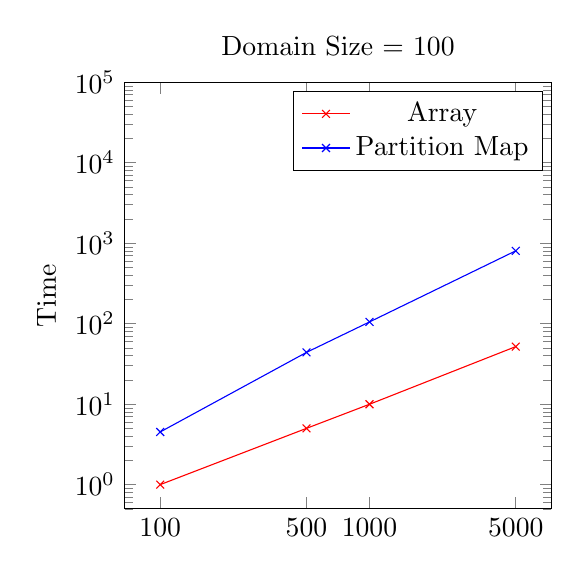
\begin{tikzpicture}
\begin{loglogaxis}[% xlabel=Merges
                    ylabel=Time
                  , title={Domain Size = 100}
                  , width=7cm
                  , height=7cm
                  , ymin=0.5
                  , ymax=1e5
                  %, ytick={0,1,10,100,1000,10000}
                  , xtick=data
                  , xticklabels={100,500,1000, 5000}
                  , xticklabel style={anchor=north}
                  ]
\addplot[color=red,mark=x] coordinates {
  (100, 1.00)
  (500, 5.00)
  (1000, 9.96)
  (5000, 51.84)
};
\addplot[color=blue,mark=x] coordinates {
  (100, 4.51)
  (500, 43.95)
  (1000, 104.99)
  (5000, 803.01)
};
\legend{Array, Partition Map}
\end{loglogaxis}
\end{tikzpicture}
&
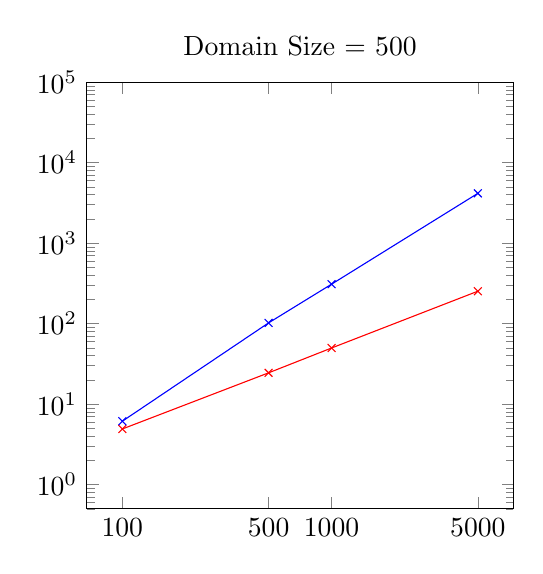
\begin{tikzpicture}
\begin{loglogaxis}[% xlabel=Merges
                  %, ylabel=Time
                    title={Domain Size = 500}
                  , width=7cm
                  , height=7cm
                  , ymin=0.5
                  , ymax=1e5
                  %, ytick={0,1,10,100,1000,10000}
                  , xtick=data
                  , xticklabels={100,500,1000, 5000}
                  , xticklabel style={anchor=north}
                  ]
\addplot[color=red,mark=x] coordinates {
  (100, 4.91)
  (500, 24.48)
  (1000, 49.83)
  (5000, 252.94)
};
\addplot[color=blue,mark=x] coordinates {
  (100, 6.13)
  (500, 102.19)
  (1000, 309.29)
  (5000, 4157.19)
};
\end{loglogaxis}
\end{tikzpicture}
\\ %
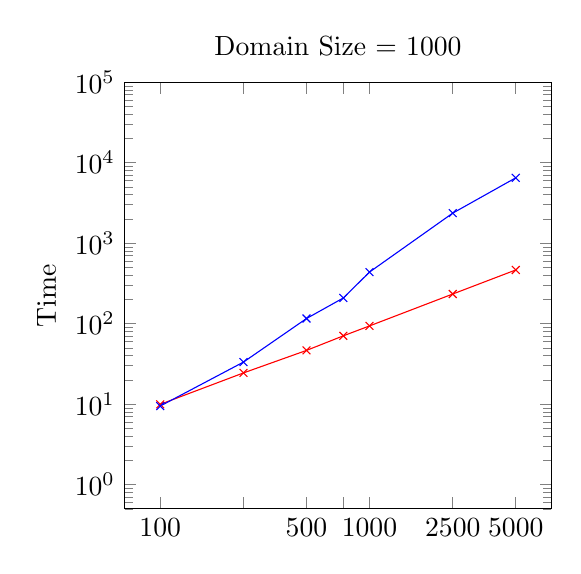
\begin{tikzpicture}
\begin{loglogaxis}[% xlabel=Merges
                    ylabel=Time
                  , title={Domain Size = 1000}
                  , width=7cm
                  , height=7cm
                  , ymin=0.5
                  , ymax=1e5
                  , xtick=data
                  , xticklabels={100,,500,,1000,2500,5000}
                  , xticklabel style={anchor=north}
                  ]
\addplot[color=red,mark=x] coordinates {
  (100,	9.94)
  (250,	24.43)
  (500,	46.49)
  (750,	70.56)
  (1000, 93.67)
  (2500, 233.43)
  (5000, 464.53)
};

\addplot[color=blue,mark=x] coordinates {
  (100, 9.46)
  (250, 33.31)
  (500, 115.74)
  (750, 208.37)
  (1000, 436.95)
  (2500, 2362.05)
  (5000, 6484.38)
};
\end{loglogaxis}
\end{tikzpicture}
&
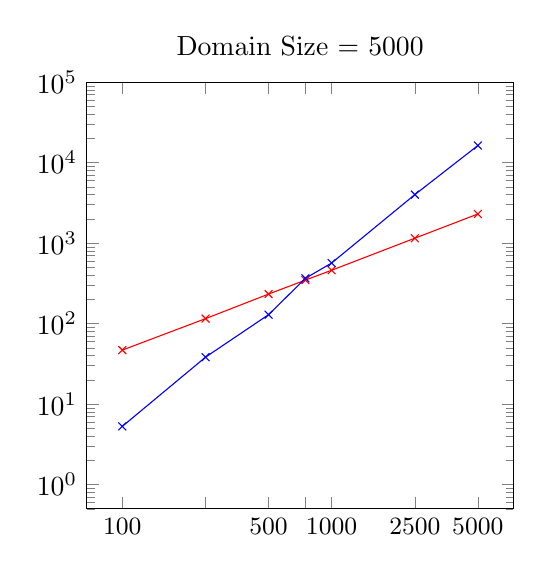
\begin{tikzpicture}
\begin{loglogaxis}[% xlabel=Merges
                  %, ylabel=Time
                    title={Domain Size = 5000}
                  , width=7cm
                  , height=7cm
                  , ymin=0.5
                  , ymax=1e5
                  , xtick=data
                  , xticklabels={100,,500,,1000,2500,5000}
                  , xticklabel style={anchor=north,font=\small}
                  ]
\addplot[color=red,mark=x] coordinates {
  (100,	46.90)
  (250,	115.44)
  (500,	233.01)
  (750,	347.75)
  (1000,	460.53)
  (2500,	1152.19)
  (5000,	2303.18)
};

\addplot[color=blue,mark=x] coordinates {
  (100, 5.29)
  (250, 38.36)
  (500, 129.29)
  (750, 365.72)
  (1000, 566.07)
  (2500, 4009.40)
  (5000, 16318.09)
};
\end{loglogaxis}
\end{tikzpicture}

\end{tabular}
\end{center}
\end{adjustwidth}
\end{figure}

The immediate take away is that in only a limited set of scenarios do
partition maps outperform the naive approach.
But there are a couple points to consider.
First, the array sizes that we are comparing against are relatively small
and in all cases the entire data set, including the domains to merge,
can fit onto a CPU-cache.
Therefore determining the two values to add is pretty fast and difficult for
partition maps to compete against.

Second,
notice that for a given domain size,
the time increases proportional to the number of merges, as expected.
But the time also increases as the domain increase: the curve rises.
Partition maps do not exhibit the same behavior,
rather their curve tilts!
Consequently, for a small number of merges partition maps will be faster
than arrays.

Regardless,
the reader is probably disappointed;
she was promised an interesting data-structure but in only a limited
case does it actually prove to be useful.
Fortunately, not everything is lost.
Here is another benchmark where we lower the expected size of the range
to 1.5.
The take-away message is that the complexity of the computation matters;
if it is simple, then partition maps can help.

\begin{figure}[!ht]
  \caption{Comparing Arrays vs Partition Map, $E[|R|] = 1.5$.}
\begin{adjustwidth}{-0.5in}{}
\begin{center}
\begin{tabular}{rl}
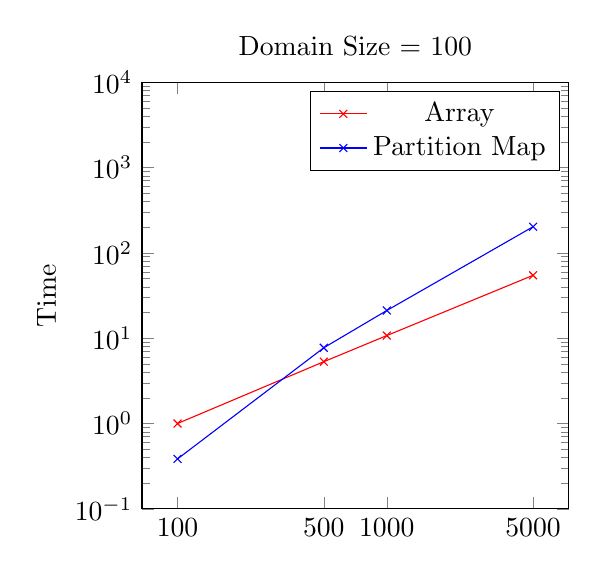
\begin{tikzpicture}
\begin{loglogaxis}[% xlabel=Merges
                    ylabel=Time
                  , width=7cm
                  , height=7cm
                  , title={Domain Size = 100}
                  , ymin=0.1
                  , ymax=1e4
                  %, ytick={0,1,10,100,1000,10000}
                  , xtick=data
                  , xticklabels={100,500,1000,5000}
                  , xticklabel style={anchor=north}
                  ]
\addplot[color=red,mark=x] coordinates {
  (100, 1.000000)
  (500, 5.301532)
  (1000, 10.727934)
  (5000, 54.528427)
};
\addplot[color=blue,mark=x] coordinates {
  (100, 0.384605)
  (500, 7.720924)
  (1000, 21.098390)
  (5000, 202.140966)
};
\legend{Array, Partition Map}
\end{loglogaxis}
\end{tikzpicture}
&
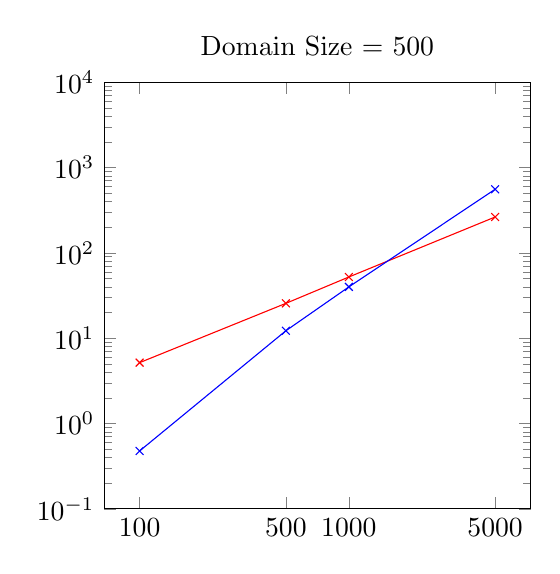
\begin{tikzpicture}
\begin{loglogaxis}[% xlabel=Merges
                  %, ylabel=Time
                    width=7cm
                  , height=7cm
                  , title={Domain Size = 500}
                  , ymin=0.1
                  , ymax=1e4
                  %, ytick={0,1,10,100,1000,10000}
                  , xtick=data
                  , xticklabels={100,500,1000, 5000}
                  , xticklabel style={anchor=north}
                  ]
\addplot[color=red,mark=x] coordinates {
  (100, 5.169652)
  (500, 25.593588)
  (1000, 52.150701)
  (5000, 263.246755)
};
\addplot[color=blue,mark=x] coordinates {
  (100, 0.476895)
  (500, 12.223261)
  (1000, 39.914200)
  (5000, 555.920561)
};
\end{loglogaxis}
\end{tikzpicture}
\\ %
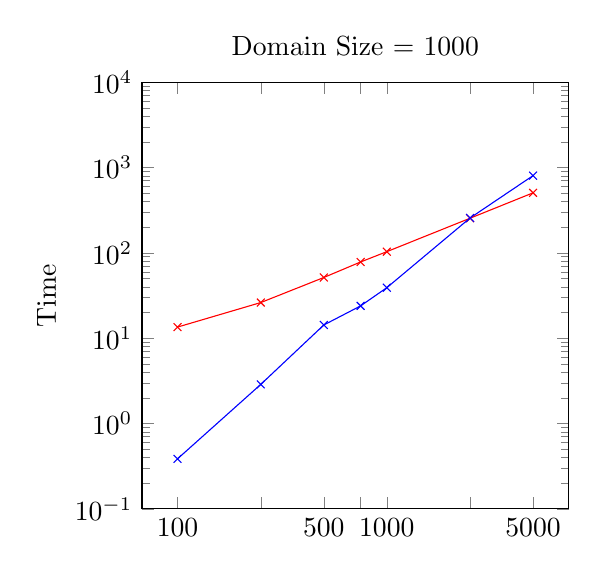
\begin{tikzpicture}
\begin{loglogaxis}[% xlabel=Merges
                    ylabel=Time
                  , width=7cm
                  , height=7cm
                  , title={Domain Size = 1000}
                  , ymin=0.1
                  , ymax=1e4
                  , xtick=data
                  , xticklabels={100,,500,,1000,,5000}
                  , xticklabel style={anchor=north}
                  ]
\addplot[color=red,mark=x] coordinates {
  (100, 13.491563)
  (250, 26.161475)
  (500, 51.429387)
  (750, 78.238188)
  (1000, 103.226765)
  (2500, 254.535955)
  (5000, 505.253505)
};

\addplot[color=blue,mark=x] coordinates {
  (100, 0.385644)
  (250, 2.876038)
  (500, 14.275182)
  (750, 23.910306)
  (1000, 39.036604)
  (2500, 256.074766)
  (5000, 803.758567)
};
\end{loglogaxis}
\end{tikzpicture}
&
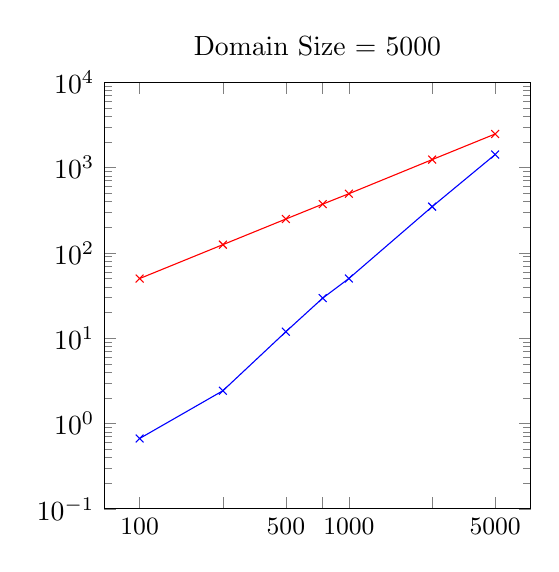
\begin{tikzpicture}
\begin{loglogaxis}[% xlabel=Merges
                  %, ylabel=Time
                    title={Domain Size = 5000}
                  , width=7cm
                  , height=7cm
                  , ymin=0.1
                  , ymax=1e4
                  , xtick=data
                  , xticklabels={100,,500,,1000,,5000}
                  , xticklabel style={anchor=north,font=\small}
                  ]
\addplot[color=red,mark=x] coordinates {
  (100, 49.960021)
  (250, 124.778946)
  (500, 249.161604)
  (750, 372.529984)
  (1000, 493.225208)
  (2500, 1237.998442)
  (5000, 2472.004413)
};

\addplot[color=blue,mark=x] coordinates {
  (100, 0.667445)
  (250, 2.420820)
  (500, 11.919003)
  (750, 29.504543)
  (1000, 50.034917)
  (2500, 347.868899)
  (5000, 1419.972482)
};
\end{loglogaxis}
\end{tikzpicture}

\end{tabular}
\end{center}
\end{adjustwidth}
\end{figure}


Lastly, observe that there is a slight kink in the partition maps
performance trend\footnote{The reason why I included 250 and 750 merges.}.
I am not certain of the exact cause
as I have not figured out an adequate model of this running time.
I think that it represents something like a phase transition;
at some point the relationship of
length of the list storing the interval and values,
versus the length of the intervals becomes more and then less
favorable for the operation.
I only highlight it because I have seen this odd behavior before and to
emphasize that a better understanding of Algorithm \ref{Alm4} is needed.

\subsection{Details}
\subsubsection{Interval representation}

Given that the domain is limited.
It is probable that for reasonable problems,
it is much smaller than the set of representable integers ($2^{32}$ or $2^{64}$).
Furthermore,
one of the big practical burdens of this algorithm is the storage of the intervals
as pairs.
Creating a pair requires extra allocations, or a pointer to the data.

One implementation shortcut that I use is to pack the interval into one integer,
where the start value occupies the upper half of the bits,
and the end occupies the lower.
In the 64-bit case, store $I = [s,e]$ as  $s \cdot 2^{32}+e$.
Aside from less allocations,
this also makes comparing intervals much faster
and a better version of Algorithm \ref{Alm2} can be implemented that
takes only one comparison to see if two intervals are equal.

\section{Conclusion and open questions}

This is still a work in progress,
and I am do not think that the current method and implementation is the best
one possible.
A big motivation for publishing and exposing this work is to gather feedback.
I have tried my best to find connections to other approaches,
and perhaps this technique is well understood and studied under a different name.
I have also not been successful in providing proofs of various claims,
nor even improve their somewhat unsatisfactory worst case
performance.%\footnote{$O(m^{2}n^{2})$ can easily be worse than $O(|D|)$ especially because
%of modern hardware configurations.}.

None-the-less, I have found this technique useful and wanted to reach out to a
broader community.
I will close by describing what I see to be the interesting problems remaining.
I have divided the problems into a practical and theoretical categories.

\subsection{Practical}
\subsubsection{Is there a fully implicit form of partition maps?}

The methods describe here use nested lists to represent the final association,
and the implementation is in OCaml,
a functional garbage-collected language.
The cost of managing the pointers for our data-structure,
is handled by the garbage-collector\footnote{
  In my use case the program spends around 25\% of the running time in the GC.},
and perhaps a hand-tuned solution might do better.
But such a solution would rely upon carefully managing space for
the sets of the partition and values (or pointers to them).
This leads to an important question of whether the entire arrangement may be
encoded in an implicit form.
This approach could alleviate the current implementations cache-unfriendliness.

In our custom implementation of intervals, we encoded the start and end
within a single integer because the size of the domain was much smaller
than what is ultimately representable by even half a 32bit word.
But this leaves open the question of whether we can encode even more state
into a given word.

\subsubsection{SIMD}

If a good implicit representation is possible where essentially arrays of
integers are used to represent the sets of a partition and pointers to values.
The operations that merge more than one partition map could be bottlenecked
at comparing integers,
in this case SIMD operations could be helpful.

This would be particularly useful to functions that merge more than 2
partition maps.

\subsection{Theoretical}

\subsubsection{Define simple and bounded}

The current work leaves these terms,
used to describe when one might use partition maps,
loosely defined,
and gives examples as opposed to practical guidance.
Consequently,
the cost of evaluating the merge operation $f$ does not permeate
the run time analysis,
of the total partition map merge.

\subsubsection{Do we have to traverse the whole accumulator?}

What techniques can we leverage to make adding to the accumulator
faster than traversing the entire list.
At the moment we are only asking for an equality test.
But if we were to ask for a comparator could we use that to arrange the values,
and the sets that they point at,
to preserve fast merging yet provide faster ways to detect duplicate elements
of the range and then preserve boundedness.

\subsubsection{Hashing sets within a partition?}

Does there exist a way to efficiently hash a set within a partition?
The current work uses an association list to store data, but being able to
hash a set would open up the possibility of using hash table like
or Patricia tree like data structures (as previously
described\cite{Okasaki1998}).
For most purposes,
we can expect that $|D|<2^{64}$,
so a 64-bit word size would be sufficient.
But we want two properties for this function.
First, efficient computation,
we do not have the resources for a cryptographic secure hash,
as we would be competing against integer comparisons.
And second,
an ability to preserve intersections and set-difference operations.
This last request,
seems particularly daunting,
so perhaps this approach is dubious.

\section{Acknowledgments}

This research was initiated and performed while the author was employed by
Mount Sinai and previously supported by the Parker Institute for Cancer
Immunotherapy.
The author is indebted to helpful discussions with Sebastian Mondet.

\clearpage

\bibliographystyle{plain}
\bibliography{note}

\end{document}
